\documentclass[11pt,a4paper]{article}

% ---------------------------------------------------------------
% Tipografia: Palatino, versalete, uma cor de destaque (bordô)
% ---------------------------------------------------------------
\usepackage[utf8]{inputenc}
\usepackage[T1]{fontenc}
\usepackage[brazil]{babel}
\usepackage[sc,osf]{mathpazo}
\usepackage{microtype}
\usepackage[top=2.4cm, bottom=2.6cm, left=2.6cm, right=2.6cm]{geometry}
\usepackage{amsmath}
\usepackage{amssymb}
\usepackage{xcolor}
\usepackage{tcolorbox}
\tcbuselibrary{skins, breakable}
\usepackage{enumitem}
\usepackage{booktabs}
\usepackage{array}
\usepackage{tabularx}
\usepackage{needspace}
\usepackage{hyperref}
\usepackage{tikz}
\usepackage{pgfplots}
\usepackage{comment}
% Para anexar as resolu\c{c}\~oes manuscritas no fim (ver o rodap\'e
% deste arquivo), descomentar a linha abaixo:
% \usepackage{pdfpages}
\pgfplotsset{compat=1.18}
\usetikzlibrary{arrows.meta, patterns, decorations.pathmorphing}

\definecolor{vinho}{RGB}{122, 27, 42}
\definecolor{grafite}{RGB}{70, 70, 70}
\hypersetup{colorlinks=true, linkcolor=vinho, urlcolor=vinho}

\linespread{1.06}
\setlength{\parindent}{0pt}
\setlength{\parskip}{0.45em}

% ---------------------------------------------------------------
% Formatação das questões
% ---------------------------------------------------------------
\newcommand{\selosala}{{\small\scshape\color{vinho}[fazer em sala]}\ }
\newcommand{\selobonus}{{\small\scshape\color{vinho}[sala --- b\^onus]}\ }
\newcommand{\fonte}[1]{{\small\scshape\color{grafite}#1}}

\newenvironment{questao}[2]{%
  \needspace{6\baselineskip}
  \par\addvspace{1.6em}
  {\large\bfseries\color{vinho}Quest\~ao #1}\hfill #2\\[-0.55em]
  {\color{black!25}\rule{\linewidth}{0.4pt}}
  \par\nobreak\smallskip
}{\par\addvspace{0.4em}}

\newcommand{\parte}[1]{%
  \needspace{7\baselineskip}
  \vspace{1.8em}
  {\Large\bfseries #1}\\[-0.55em]
  {\color{black!30}\rule{\linewidth}{0.5pt}}
  \par\nobreak\smallskip
}

\newtcolorbox{painel}{blanker, breakable, left=12pt,
  borderline west={1.4pt}{0pt}{black!30},
  before skip=11pt, after skip=11pt}

\newcommand{\redesenhada}{%
  {\small\itshape (Figura redesenhada --- n\~ao \'e a arte original da
  prova.)}}

\setlist[enumerate,1]{label=\textbf{\alph*)}, leftmargin=2em, nosep}

% ---------------------------------------------------------------
\begin{document}
% ---------------------------------------------------------------

% ---------------------------------------------------------------
% TÍTULO
% ---------------------------------------------------------------
\thispagestyle{empty}

{\scshape\color{vinho}cursinho solid\'ario \,\textperiodcentered\, f\'isica}\\[-0.5em]
{\color{vinho}\rule{\linewidth}{1.6pt}}\\[0.9em]
{\huge\bfseries Lista de Quest\~oes}\\[0.35em]
{\LARGE Trabalho e Energia}\\[0.7em]
{\itshape\color{grafite}Quest\~oes de ENEM e de vestibulares
(UTFPR, UFMG, UFF, UERJ e outros)}
\hfill {\color{grafite}2026}\\[-0.3em]
{\color{black!30}\rule{\linewidth}{0.5pt}}

\vspace{1.0em}

\begin{painel}

\begin{itemize}[nosep, leftmargin=1.5em]
  \item Todas as quest\~oes s\~ao de provas antigas. A fonte e o ano
        est\~ao do lado do n\'umero.
  \item Em toda a lista, adotar $g = 10$ m/s\textsuperscript{2},
        salvo indica\c{c}\~ao contr\'aria no enunciado.
  \item Come\c{c}ar por Q1, Q5 e Q10 (uma de cada ideia: trabalho,
        teorema $W = \Delta E_c$ e conserva\c{c}\~ao); Q13 \'e o
        treino de energia dissipada pelo atrito.
  \item Q19 e Q20 s\~ao desafios.
  \item No fim da lista tem o gabarito comentado, com a conta de
        todas as quest\~oes num\'ericas.
\end{itemize}
\end{painel}

\newpage

{\renewcommand{\arraystretch}{1.25}
\begin{tabular}{@{}clll@{}}
  \multicolumn{4}{@{}l}{{\scshape\color{vinho}mapa da lista}}\\
  \addlinespace[2pt]
  \toprule
  \# & Fonte & Tema & Onde \\
  \midrule
  1  & UFF                & Trabalho e o \^angulo da for\c{c}a          & \textbf{sala} \\
  2  & UFMG 2003          & Trabalho do peso $\times$ trajet\'oria       & \textbf{sala} \\
  3  & UFSCar             & Velocidade constante e trabalho total       & casa \\
  4  & UNIRIO             & $E_c$ e o quadrado da velocidade            & casa \\
  5  & FGV                & Teorema $W = \Delta E_c$ (num\'erica)       & \textbf{sala} \\
  6  & ESCS DF            & Trabalho dos m\'usculos no salto            & casa \\
  7  & UFF                & \'Area do gr\'afico $F \times x$            & \textbf{sala} \\
  8  & ENEM 2011          & Conserva\c{c}\~ao: salto com vara           & \textbf{sala (b\^onus)} \\
  9  & UERJ               & Queda: dobrar a velocidade de impacto       & casa \\
  10 & UERJ               & Conserva\c{c}\~ao: bola no ar (num\'erica)  & \textbf{sala} \\
  11 & ENEM 2018          & Energia el\'astica ($kx^2/2$)               & \textbf{sala} \\
  12 & ENEM 2022          & Energia dissipada na colis\~ao              & \textbf{sala (b\^onus)} \\
  13 & UNIFOR CE          & Energia mec\^anica perdida na queda         & \textbf{sala} \\
  14 & UFLA MG            & Mola $+$ atrito $+$ rampa                   & casa \\
  15 & UTFPR Ver\~ao 2026 & Pot\^encia do guindaste ($P = Fv$)          & casa \\
  16 & ENEM 2016          & Pot\^encia da usina de Itaipu               & casa \\
  17 & UTFPR Inverno 2023 & Rendimento e kWh (fotovoltaico)             & \textbf{sala} \\
  18 & UTFPR Ver\~ao 2025 & Energia em kWh (fotovoltaico)               & casa \\
  19 & ENEM 2015          & Desafio: carro solar                        & casa \\
  20 & ENEM 2019          & Desafio: disco de Maxwell                   & casa \\
  \bottomrule
\end{tabular}}

\newpage

% ===================================================================
\parte{Parte I --- Trabalho de uma For\c{c}a}
% ===================================================================

\begin{questao}{1}{\fonte{UFF}}
\selosala
Um motorista empurra um carro sem combust\'ivel at\'e um posto mais
pr\'oximo. Na primeira metade do trajeto, o motorista empurra o carro
por tr\'as (situa\c{c}\~ao I) e na segunda metade do trajeto ele o
empurra pelo lado (situa\c{c}\~ao II).

\begin{center}
\begin{tikzpicture}[scale=1.0]
  % ---- Situa\c{c}\~ao I ----
  \begin{scope}
    \draw[dashed, black!55] (-1.6,0) -- (4.6,0);
    \draw[thick, fill=black!5, rounded corners=4pt]
      (0.9,-0.55) rectangle (3.6,0.55);
    \draw[thick] (1.5,-0.55) -- (1.5,0.55);
    \draw[thick] (3.0,-0.55) -- (3.0,0.55);
    \draw[thick, fill=black!25] (0.35,0) circle (0.2);
    \draw[-{Stealth[length=3mm]}, very thick] (-0.9,0) -- (0.1,0)
      node[midway, above] {$\vec{F}$};
    \node[anchor=north] at (2.25,-0.75) {\small Situa\c{c}\~ao I};
  \end{scope}
  % ---- Situa\c{c}\~ao II ----
  \begin{scope}[yshift=-3.4cm]
    \draw[dashed, black!55] (-1.6,0) -- (4.6,0);
    \draw[thick, fill=black!5, rounded corners=4pt]
      (0.9,-0.55) rectangle (3.6,0.55);
    \draw[thick] (1.5,-0.55) -- (1.5,0.55);
    \draw[thick] (3.0,-0.55) -- (3.0,0.55);
    % motorista ao lado do carro
    \draw[thick, fill=black!25] (0.42,-1.30) circle (0.2);
    % linha de refer\^encia paralela ao movimento
    \draw[dashed, black!55] (0.62,-1.20) -- (2.55,-1.20);
    % for\c{c}a inclinada de theta
    \draw[-{Stealth[length=3mm]}, very thick] (0.62,-1.20) -- (1.85,-0.44)
      node[pos=0.30, above, sloped] {$\vec{F}$};
    \draw[black!70] (1.52,-1.20) arc (0:32:0.90);
    \node at (1.62,-0.99) {\small $\theta$};
    \node[anchor=north] at (2.25,-1.75) {\small Situa\c{c}\~ao II};
  \end{scope}
\end{tikzpicture}\\
\redesenhada
\end{center}

Nas figuras, est\'a tamb\'em representada a for\c{c}a $\vec{F}$ que o
motorista faz sobre o carro, em cada caso. Sabendo que a intensidade
desta for\c{c}a \'e constante e a mesma nas duas situa\c{c}\~oes, \'e
correto afirmar que:
\begin{enumerate}
  \item o trabalho realizado pelo motorista \'e maior na
        situa\c{c}\~ao II.
  \item o trabalho realizado pelo motorista \'e o mesmo nas duas
        situa\c{c}\~oes.
  \item a energia transferida para o carro pelo motorista \'e maior na
        situa\c{c}\~ao I.
  \item a energia transferida para o carro pelo motorista \'e menor na
        situa\c{c}\~ao I.
  \item o trabalho realizado pelo motorista na situa\c{c}\~ao I \'e
        menor do que a energia por ele transferida para o carro na
        situa\c{c}\~ao II.
\end{enumerate}
\end{questao}

\begin{questao}{2}{\fonte{UFMG 2003}}
\selosala
Para chegar ao segundo andar de sua escola, Andr\'e pode subir por uma
escada ou por uma rampa. Se subir pela escada, com velocidade
constante, ele demora 10 s; no entanto, se for pela rampa, com a mesma
velocidade, leva 15 s.

Sejam $W_E$ o trabalho realizado e $P_E$ a pot\^encia m\'edia
desenvolvida por Andr\'e para ir ao segundo andar pela escada. Indo
pela rampa, esses valores s\~ao, respectivamente, $W_R$ e $P_R$.
Despreze perdas de energia por atrito. Com base nessas
informa\c{c}\~oes, \'e correto afirmar que:
\begin{enumerate}
  \item $W_E \neq W_R$ \ e \ $P_E < P_R$
  \item $W_E \neq W_R$ \ e \ $P_E > P_R$
  \item $W_E = W_R$ \ e \ $P_E < P_R$
  \item $W_E = W_R$ \ e \ $P_E > P_R$
\end{enumerate}
\end{questao}

\begin{questao}{3}{\fonte{UFSCar}}
Nas provas de longa e m\'edia dist\^ancia do atletismo, os corredores
mant\^em sua velocidade constante durante a maior parte do tempo. A
partir dessa constata\c{c}\~ao, um estudante de f\'isica afirma que,
durante esse tempo, os atletas n\~ao gastam energia porque a energia
cin\'etica deles n\~ao varia. Essa afirma\c{c}\~ao \'e:
\begin{enumerate}
  \item verdadeira, pois os corredores se mant\^em em movimento sem
        esfor\c{c}o, por in\'ercia.
  \item verdadeira do ponto de vista da f\'isica, mas falsa do ponto
        de vista da biologia.
  \item falsa, porque a energia cin\'etica do atleta n\~ao tem
        rela\c{c}\~ao com o esfor\c{c}o muscular que ele desenvolve.
  \item falsa, pois a energia cin\'etica s\'o se mant\'em constante
        gra\c{c}as ao trabalho da for\c{c}a muscular do atleta.
  \item verdadeira, porque o trabalho da resultante das for\c{c}as que
        atuam sobre o atleta \'e nulo.
\end{enumerate}
\end{questao}

% ===================================================================
\parte{Parte II --- Energia Cin\'etica e o Teorema $W = \Delta E_c$}
% ===================================================================

\begin{questao}{4}{\fonte{UNIRIO}}
Quando a velocidade de um m\'ovel duplica, sua energia cin\'etica:
\begin{enumerate}
  \item reduz-se a um quarto do valor inicial.
  \item reduz-se \`a metade.
  \item fica multiplicada por $\sqrt{2}$.
  \item duplica.
  \item quadruplica.
\end{enumerate}
\end{questao}

\begin{questao}{5}{\fonte{FGV}}
\selosala
Em alguns pa\'ises da Europa, os radares fotogr\'aficos das rodovias,
al\'em de detectarem a velocidade instant\^anea dos ve\'iculos, s\~ao
capazes de determinar a velocidade m\'edia desenvolvida pelos
ve\'iculos entre dois radares consecutivos.

Considere dois desses radares instalados em uma rodovia retil\'inea e
horizontal. A velocidade instant\^anea de certo autom\'ovel, de
1\,500 kg de massa, registrada pelo primeiro radar foi de 72 km/h. Um
minuto depois, o radar seguinte acusou 90 km/h para o mesmo
autom\'ovel.

O trabalho realizado pela resultante das for\c{c}as agentes sobre o
autom\'ovel foi, em joules, mais pr\'oximo de
\begin{enumerate}
  \item $1{,}5 \times 10^{4}$.
  \item $5{,}2 \times 10^{4}$.
  \item $7{,}5 \times 10^{4}$.
  \item $1{,}7 \times 10^{5}$.
  \item $3{,}2 \times 10^{5}$.
\end{enumerate}
\end{questao}

\begin{questao}{6}{\fonte{ESCS DF}}
Uma pessoa resolve dar um salto vertical e, para isso, flexiona suas
pernas. No instante $t_1$ ela est\'a em repouso, agachada. O ponto C
representa seu centro de massa. No instante $t_2$ ela abandona o solo
e, a partir da\'i, todas as partes do corpo t\^em a mesma velocidade,
a do centro de massa. No instante $t_3$ o centro de massa atinge a
altura m\'axima. Entre $t_1$ e $t_2$ o centro de massa subiu uma
altura $d = 30$ cm, e entre $t_2$ e $t_3$, uma altura $h$.

\begin{center}
\begin{tikzpicture}[scale=1.25]
  % ch\~ao
  \draw[thick] (-0.2,0) -- (6.6,0);
  \fill[pattern=north east lines] (-0.2,-0.16) rectangle (6.6,0);
  % ---- instante t1: agachado ----
  \draw[thick] (1.0,0.62) circle (0.16);
  \draw[thick] (1.0,0.46) -- (1.0,0.16);
  \draw[thick] (1.0,0.16) -- (0.82,0.0);
  \draw[thick] (1.0,0.16) -- (1.20,0.0);
  \draw[thick] (1.0,0.40) -- (1.32,0.46);
  \fill (1.0,0.30) circle (0.05);
  \node[anchor=west] at (1.06,0.30) {\small C};
  \node[anchor=north] at (1.0,-0.25) {\small $t_1$};
  % ---- instante t2: deixando o solo ----
  \draw[thick] (3.2,1.10) circle (0.16);
  \draw[thick] (3.2,0.94) -- (3.2,0.36);
  \draw[thick] (3.2,0.36) -- (3.06,0.0);
  \draw[thick] (3.2,0.36) -- (3.36,0.0);
  \draw[thick] (3.2,0.86) -- (3.06,1.34);
  \draw[thick] (3.2,0.86) -- (3.38,1.34);
  \fill (3.2,0.60) circle (0.05);
  \node[anchor=west] at (3.26,0.60) {\small C};
  \node[anchor=north] at (3.2,-0.25) {\small $t_2$};
  % ---- instante t3: altura m\'axima ----
  \draw[thick] (5.4,1.70) circle (0.16);
  \draw[thick] (5.4,1.54) -- (5.4,0.96);
  \draw[thick] (5.4,0.96) -- (5.26,0.60);
  \draw[thick] (5.4,0.96) -- (5.56,0.60);
  \draw[thick] (5.4,1.46) -- (5.26,1.94);
  \draw[thick] (5.4,1.46) -- (5.58,1.94);
  \fill (5.4,1.20) circle (0.05);
  \node[anchor=west] at (5.46,1.20) {\small C};
  \node[anchor=north] at (5.4,-0.25) {\small $t_3$};
  % ---- cotas ----
  \draw[dashed, black!55] (1.0,0.30) -- (6.10,0.30);
  \draw[dashed, black!55] (3.2,0.60) -- (6.10,0.60);
  \draw[dashed, black!55] (5.4,1.20) -- (6.10,1.20);
  \draw[<->] (6.00,0.30) -- (6.00,0.60) node[midway, right] {\small $d$};
  \draw[<->] (6.35,0.60) -- (6.35,1.20) node[midway, right] {\small $h$};
  \draw[dashed, black!55] (6.10,0.60) -- (6.45,0.60);
  \draw[dashed, black!55] (6.10,1.20) -- (6.45,1.20);
\end{tikzpicture}\\
\redesenhada
\end{center}

A massa da pessoa vale 50 kg e o trabalho total de seus m\'usculos, no
intervalo de $t_1$ a $t_2$, foi $W = 450$ J. O valor da altura $h$ \'e
igual a:
\begin{enumerate}
  \item 30 cm
  \item 60 cm
  \item 90 cm
  \item 1,5 m
  \item 1,2 m
\end{enumerate}
\end{questao}

\begin{questao}{7}{\fonte{UFF}}
\selosala
O gr\'afico mostra o comportamento da intensidade da \'unica for\c{c}a
que age sobre uma part\'icula, em fun\c{c}\~ao de sua posi\c{c}\~ao
($x$) ao longo de uma trajet\'oria retil\'inea horizontal. A
part\'icula se desloca desde $x = -L$, sempre no sentido positivo de
sua trajet\'oria.

\begin{center}
\begin{tikzpicture}[scale=1.0]
  % eixos
  \draw[-{Stealth[length=2.5mm]}] (-2.6,0) -- (5.3,0)
    node[anchor=west] {\small $x$};
  \draw[-{Stealth[length=2.5mm]}] (0,-0.5) -- (0,3.2)
    node[anchor=south] {\small For\c{c}a};
  % curva: constante F de -L a L, depois cresce ate 2F em 2L
  \draw[very thick] (-2,1.3) -- (2,1.3) -- (4,2.6);
  % linhas de chamada
  \draw[dashed, black!55] (-2,0) -- (-2,1.3);
  \draw[dashed, black!55] (2,0) -- (2,1.3);
  \draw[dashed, black!55] (4,0) -- (4,2.6);
  \draw[dashed, black!55] (0,2.6) -- (4,2.6);
  \draw[dashed, black!55] (0,1.3) -- (-2,1.3);
  % r\'otulos
  \node[anchor=north] at (-2,-0.08) {\small $-L$};
  \node[anchor=north east] at (-0.02,-0.08) {\small $0$};
  \node[anchor=north] at (2,-0.08) {\small $L$};
  \node[anchor=north] at (4,-0.08) {\small $2L$};
  \node[anchor=east] at (-0.08,1.3) {\small $F$};
  \node[anchor=east] at (-0.08,2.6) {\small $2F$};
\end{tikzpicture}\\
\redesenhada
\end{center}

Nestas condi\c{c}\~oes, \'e correto afirmar que:
\begin{enumerate}
  \item a varia\c{c}\~ao da energia cin\'etica da part\'icula \'e
        \textbf{menor} entre as posi\c{c}\~oes $x = -L$ e $x = L$ do
        que entre as posi\c{c}\~oes $x = 0$ e $x = 2L$.
  \item a varia\c{c}\~ao da energia cin\'etica da part\'icula \'e
        \textbf{nula} entre as posi\c{c}\~oes $x = -L$ e $x = L$.
  \item a varia\c{c}\~ao da energia cin\'etica da part\'icula \'e
        \textbf{maior} entre as posi\c{c}\~oes $x = 0$ e $x = L$ do
        que entre as posi\c{c}\~oes $x = L$ e $x = 2L$.
  \item a energia cin\'etica da part\'icula diminui entre as
        posi\c{c}\~oes $x = -L$ e $x = 0$.
  \item a energia cin\'etica da part\'icula diminui entre as
        posi\c{c}\~oes $x = L$ e $x = 2L$.
\end{enumerate}
\end{questao}

% ===================================================================
\parte{Parte III --- Energia Potencial e Conserva\c{c}\~ao}
% ===================================================================

\begin{questao}{8}{\fonte{ENEM 2011 --- Q86}}
\selobonus
Uma das modalidades presentes nas olimp\'iadas \'e o salto com vara.
As etapas de um dos saltos de um atleta est\~ao representadas na
figura:

\begin{center}
\begin{tikzpicture}[scale=0.95]
  % ---------- Etapa I ----------
  \begin{scope}
    \draw[black!45] (0,0) rectangle (3.6,2.2);
    \node[anchor=north] at (1.8,2.14) {\small Etapa I};
    \draw[thick] (0.25,0.35) -- (3.35,0.35);
    \draw[thick] (1.05,1.25) circle (0.17);
    \draw[thick] (1.05,1.08) -- (1.05,0.72);
    \draw[thick] (1.05,0.72) -- (0.85,0.35);
    \draw[thick] (1.05,0.72) -- (1.30,0.35);
    \draw[thick] (1.05,1.00) -- (1.35,1.10);
    \draw[line width=1.7pt, black!55] (0.85,1.08) -- (2.95,1.18);
    \node[anchor=north] at (1.8,-0.04) {\scriptsize Atleta corre com a vara};
  \end{scope}
  % ---------- Etapa II ----------
  \begin{scope}[xshift=3.9cm]
    \draw[black!45] (0,0) rectangle (3.6,2.2);
    \node[anchor=north] at (1.8,2.14) {\small Etapa II};
    \draw[thick] (0.25,0.35) -- (3.35,0.35);
    \draw[line width=1.7pt, black!55] (3.05,0.37) -- (1.00,1.15);
    \draw[thick] (0.80,1.32) circle (0.17);
    \draw[thick] (0.80,1.15) -- (0.80,0.72);
    \draw[thick] (0.80,0.72) -- (0.62,0.35);
    \draw[thick] (0.80,0.72) -- (1.02,0.35);
    \draw[thick] (0.80,1.10) -- (1.06,1.20);
    \node[anchor=north] at (1.8,-0.04) {\scriptsize Atleta apoia a vara no ch\~ao};
  \end{scope}
  % ---------- Etapa III ----------
  \begin{scope}[yshift=-3.3cm]
    \draw[black!45] (0,0) rectangle (3.6,2.2);
    \node[anchor=north] at (1.8,2.14) {\small Etapa III};
    \draw[thick] (0.25,0.35) -- (3.35,0.35);
    \draw[line width=1.7pt, black!55] (1.85,0.35) -- (1.85,1.28);
    \draw[thick] (2.12,1.44) circle (0.17);
    \draw[thick] (1.95,1.42) -- (1.52,1.34);
    \draw[thick] (1.52,1.34) -- (1.26,1.18);
    \draw[thick] (1.52,1.34) -- (1.28,1.50);
    \draw[thick] (1.74,1.38) -- (1.84,1.16);
    \node[anchor=north] at (1.8,-0.04) {\scriptsize Atleta atinge certa altura};
  \end{scope}
  % ---------- Etapa IV ----------
  \begin{scope}[xshift=3.9cm, yshift=-3.3cm]
    \draw[black!45] (0,0) rectangle (3.6,2.2);
    \node[anchor=north] at (1.8,2.14) {\small Etapa IV};
    \draw[thick] (0.25,0.35) -- (3.35,0.35);
    \draw[thick, fill=black!12] (0.80,0.35) rectangle (2.80,0.80);
    \draw[thick] (1.22,1.04) circle (0.17);
    \draw[thick] (1.39,1.02) -- (1.95,1.02);
    \draw[thick] (1.95,1.02) -- (2.30,0.90);
    \draw[thick] (1.95,1.02) -- (2.28,1.16);
    \draw[thick] (1.62,1.02) -- (1.68,1.26);
    \node[anchor=north] at (1.8,-0.04) {\scriptsize Atleta cai em um colch\~ao};
  \end{scope}
\end{tikzpicture}\\
\redesenhada
\end{center}

Desprezando-se as for\c{c}as dissipativas (resist\^encia do ar e
atrito), para que o salto atinja a maior altura poss\'ivel, ou seja, o
m\'aximo de energia seja conservada, \'e necess\'ario que
\begin{enumerate}
  \item a energia cin\'etica, representada na etapa I, seja totalmente
        convertida em energia potencial el\'astica representada na
        etapa IV.
  \item a energia cin\'etica, representada na etapa II, seja
        totalmente convertida em energia potencial gravitacional,
        representada na etapa IV.
  \item a energia cin\'etica, representada na etapa I, seja totalmente
        convertida em energia potencial gravitacional, representada na
        etapa III.
  \item a energia potencial gravitacional, representada na etapa II,
        seja totalmente convertida em energia potencial el\'astica,
        representada na etapa IV.
  \item a energia potencial gravitacional, representada na etapa I,
        seja totalmente convertida em energia potencial el\'astica,
        representada na etapa III.
\end{enumerate}
\end{questao}

\begin{questao}{9}{\fonte{UERJ}}
Um chaveiro, largado de uma varanda de altura $h$, atinge a
cal\c{c}ada com velocidade $v$. Para que a velocidade de impacto
dobrasse de valor, seria necess\'ario largar esse chaveiro de uma
altura maior, igual a:
\begin{enumerate}
  \item $2h$
  \item $3h$
  \item $4h$
  \item $6h$
\end{enumerate}
\end{questao}

\begin{questao}{10}{\fonte{UERJ}}
\selosala
Numa partida de futebol, o goleiro bate o tiro de meta e a bola, de
massa $0{,}5$ kg, sai do solo com velocidade de m\'odulo igual a
10 m/s, conforme mostra a figura.

\begin{center}
\begin{tikzpicture}[scale=1.0]
  % ch\~ao
  \draw[thick] (-0.3,0) -- (7.4,0);
  % trajet\'oria
  \draw[dashed, black!65] (0.3,0) .. controls (2.1,3.3) and (4.9,3.3)
    .. (6.6,0);
  % bola no lan\c{c}amento
  \draw[thick, fill=black!12] (0.3,0.13) circle (0.13);
  \draw[-{Stealth[length=3mm]}, very thick] (0.42,0.30) -- (1.10,1.28)
    node[midway, left] {$\vec{v}$};
  % ponto P
  \draw[thick, fill=black!12] (6.05,1.10) circle (0.13);
  \node[anchor=south west] at (6.10,1.18) {\small P};
  % jogador (esquem\'atico) sob o ponto P
  \draw[thick] (6.05,0.76) circle (0.14);
  \draw[thick] (6.05,0.62) -- (6.05,0.30);
  \draw[thick] (6.05,0.30) -- (5.90,0);
  \draw[thick] (6.05,0.30) -- (6.20,0);
  \draw[thick] (6.05,0.56) -- (6.28,0.66);
  % cota 2 m
  \draw[<->] (6.85,0) -- (6.85,1.10) node[midway, right] {\small 2 m};
  \draw[dashed, black!45] (6.18,1.10) -- (6.95,1.10);
\end{tikzpicture}\\
\redesenhada
\end{center}

No ponto P, a 2 metros do solo, um jogador da defesa advers\'aria
cabeceia a bola. Considerando $g = 10$ m/s\textsuperscript{2}, a
energia cin\'etica da bola no ponto P vale, em joules:
\begin{enumerate}
  \item 0
  \item 5
  \item 10
  \item 15
\end{enumerate}
\end{questao}

\begin{questao}{11}{\fonte{ENEM 2018 --- Q131}}
\selosala
Um projetista deseja construir um brinquedo que lance um pequeno cubo
ao longo de um trilho horizontal, e o dispositivo precisa oferecer a
op\c{c}\~ao de mudar a velocidade de lan\c{c}amento. Para isso, ele
utiliza uma mola e um trilho onde o atrito pode ser desprezado,
conforme a figura.

\begin{center}
\begin{tikzpicture}[scale=1.0]
  % trilho
  \draw[thick] (0,0) rectangle (7.0,1.0);
  \draw[thick] (0,0.12) -- (7.0,0.12);
  \draw[thick] (0,0.88) -- (7.0,0.88);
  % mola
  \draw[thick, decorate,
        decoration={coil, aspect=0.55, segment length=3.2mm,
                    amplitude=2.2mm}]
    (0.12,0.5) -- (2.35,0.5);
  % cubo
  \draw[thick, fill=black] (2.40,0.22) rectangle (3.05,0.78);
  % r\'otulos
  \node[anchor=north] at (1.2,-0.10) {\small Mola};
  \draw[-{Stealth[length=2.5mm]}] (1.2,-0.10) -- (1.4,0.42);
  \node[anchor=north] at (4.1,-0.10) {\small Trilho horizontal};
  \draw[-{Stealth[length=2.5mm]}] (4.1,-0.10) -- (4.1,0.10);
  \node[anchor=south] at (4.3,1.16) {\small Cubo};
  \draw[-{Stealth[length=2.5mm]}] (4.3,1.16) -- (3.05,0.70);
\end{tikzpicture}\\
\redesenhada
\end{center}

Para que a velocidade de lan\c{c}amento do cubo seja aumentada quatro
vezes, o projetista deve
\begin{enumerate}
  \item manter a mesma mola e aumentar duas vezes a sua
        deforma\c{c}\~ao.
  \item manter a mesma mola e aumentar quatro vezes a sua
        deforma\c{c}\~ao.
  \item manter a mesma mola e aumentar dezesseis vezes a sua
        deforma\c{c}\~ao.
  \item trocar a mola por outra de constante el\'astica duas vezes
        maior e manter a deforma\c{c}\~ao.
  \item trocar a mola por outra de constante el\'astica quatro vezes
        maior e manter a deforma\c{c}\~ao.
\end{enumerate}
\end{questao}

% ===================================================================
\parte{Parte IV --- Energia Dissipada pelo Atrito}
% ===================================================================

\begin{questao}{12}{\fonte{ENEM 2022 --- Q105}}
\selobonus
Em um aut\'odromo, os carros podem derrapar em uma curva e bater na
parede de prote\c{c}\~ao. Para diminuir o impacto de uma batida,
pode-se colocar na parede uma barreira de pneus, isso faz com que a
colis\~ao seja mais demorada e o carro retorne com velocidade
reduzida. Outra op\c{c}\~ao \'e colocar uma barreira de blocos de um
material que se deforma, tornando-a t\~ao demorada quanto a
colis\~ao com os pneus, mas que n\~ao permite a volta do carro
ap\'os a colis\~ao.

Comparando as duas situa\c{c}\~oes, como ficam a for\c{c}a m\'edia
exercida sobre o carro e a energia mec\^anica dissipada?
\begin{enumerate}
  \item A for\c{c}a \'e maior na colis\~ao com a barreira de pneus, e
        a energia dissipada \'e maior na colis\~ao com a barreira de
        blocos.
  \item A for\c{c}a \'e maior na colis\~ao com a barreira de blocos, e
        a energia dissipada \'e maior na colis\~ao com a barreira de
        pneus.
  \item A for\c{c}a \'e maior na colis\~ao com a barreira de blocos, e
        a energia dissipada \'e a mesma nas duas situa\c{c}\~oes.
  \item A for\c{c}a \'e maior na colis\~ao com a barreira de pneus, e
        a energia dissipada \'e maior na colis\~ao com a barreira de
        pneus.
  \item A for\c{c}a \'e maior na colis\~ao com a barreira de blocos, e
        a energia dissipada \'e maior na colis\~ao com a barreira de
        blocos.
\end{enumerate}
\end{questao}

\begin{questao}{13}{\fonte{UNIFOR CE}}
\selosala
Um corpo de massa $5{,}0$ kg cai verticalmente no ar, a partir do
repouso. Ap\'os percorrer $4{,}0$ m sua velocidade \'e de $6{,}0$ m/s.
Nessa queda, as mol\'eculas do corpo e do ar recebem energia que
provoca eleva\c{c}\~ao de temperatura dos corpos. De acordo com os
dados, a energia mec\^anica perdida pelo corpo vale, em joules,
(adote $g = 10$ m/s\textsuperscript{2}):
\begin{enumerate}
  \item 110
  \item 90
  \item 75
  \item 60
  \item 45
\end{enumerate}
\end{questao}

\begin{questao}{14}{\fonte{UFLA MG}}
Um corpo comprime uma mola na base de um plano inclinado, conforme
mostra a figura. Abandonando-se o sistema corpo/mola, o corpo \'e
arremessado plano acima, escorregando at\'e parar.

\begin{center}
\begin{tikzpicture}[scale=1.0]
  % ch\~ao e rampa
  \draw[thick] (-0.3,0) -- (6.6,0);
  \draw[thick] (0.5,0) -- (5.9,2.7);
  \draw[thick] (5.9,2.7) -- (5.9,0);
  \fill[pattern=north east lines, pattern color=black!45]
    (0.5,0) -- (5.9,2.7) -- (5.9,0) -- cycle;
  % mola encostada na base da rampa
  \draw[thick, decorate,
        decoration={coil, aspect=0.55, segment length=2.6mm,
                    amplitude=1.7mm}]
    (0.62,0.26) -- (1.62,0.76);
  % corpo
  \begin{scope}[shift={(1.72,0.60)}, rotate=26.6]
    \draw[thick, fill=black!12] (0,0) rectangle (0.7,0.5);
  \end{scope}
  % posicao final (tracejada) e cota h
  \begin{scope}[shift={(3.85,1.66)}, rotate=26.6]
    \draw[thick, dashed, fill=black!4] (0,0) rectangle (0.7,0.5);
  \end{scope}
  \draw[dashed, black!55] (4.25,1.87) -- (6.35,1.87);
  \draw[<->] (6.25,0) -- (6.25,1.87) node[midway, right] {\small $h$};
\end{tikzpicture}\\
\redesenhada
\end{center}

Considerando a massa do corpo 200 g, a compress\~ao da mola 4 cm, a
constante el\'astica $k = 2\,000$ N/m, $g = 10$
m/s\textsuperscript{2}, e a energia dissipada pela for\c{c}a de atrito
no deslocamento at\'e o alto do plano de $0{,}6$ J, ent\~ao a altura
vertical $h$ que o corpo atinge \'e de:
\begin{enumerate}
  \item 0,25 m
  \item 0,50 m
  \item 1,00 m
  \item 1,25 m
  \item 1,50 m
\end{enumerate}
\end{questao}

% ===================================================================
\parte{Parte V --- Pot\^encia e Rendimento}
% ===================================================================

\begin{questao}{15}{\fonte{UTFPR Ver\~ao 2026 --- Q38}}
Uma caixa de 10 kg \'e i\c{c}ada por um guindaste com uma velocidade
constante de aproximadamente 5 m/s. Desconsiderando atritos e outras
perdas e considerando que a acelera\c{c}\~ao da gravidade na
superf\'icie da Terra \'e aproximadamente 10
m/s\textsuperscript{2}, assinale a alternativa com a pot\^encia
m\'inima do motor de i\c{c}amento do guindaste necess\'aria para
realizar o i\c{c}amento descrito.
\begin{enumerate}
  \item 250 W
  \item 500 W
  \item 750 W
  \item 1\,000 W
  \item 1\,250 W
\end{enumerate}
\end{questao}

\begin{questao}{16}{\fonte{ENEM 2016 --- Q47}}
A usina de Itaipu \'e uma das maiores hidrel\'etricas do mundo em
gera\c{c}\~ao de energia. Com 20 unidades geradoras e 14\,000 MW de
pot\^encia total instalada, apresenta uma queda de $118{,}4$ m e
vaz\~ao nominal de 690 m\textsuperscript{3}/s por unidade geradora. O
c\'alculo da pot\^encia te\'orica leva em conta a altura da massa de
\'agua represada pela barragem, a gravidade local (10
m/s\textsuperscript{2}) e a densidade da \'agua (1\,000
kg/m\textsuperscript{3}). A diferen\c{c}a entre a pot\^encia
te\'orica e a instalada \'e a pot\^encia n\~ao aproveitada.
\begin{flushright}\small
Dispon\'ivel em: www.itaipu.gov.br. Acesso em: 11 maio 2013 (adaptado).
\end{flushright}

Qual \'e a pot\^encia, em MW, n\~ao aproveitada em cada unidade
geradora de Itaipu?
\begin{enumerate}
  \item 0
  \item 1,18
  \item 116,96
  \item 816,96
  \item 13\,183,04
\end{enumerate}
\end{questao}

\begin{questao}{17}{\fonte{UTFPR Inverno 2023 --- Q59}}
\selosala
A energia solar \'e uma fonte de energia renov\'avel e limpa que tem
se tornado cada vez mais importante devido \`a crescente
preocupa\c{c}\~ao com o meio ambiente e a necessidade de reduzir as
emiss\~oes de gases do efeito estufa. A instala\c{c}\~ao de sistemas
fotovoltaicos \'e uma das maneiras mais comuns de aproveitar a energia
solar para gerar eletricidade. Nos \'ultimos anos, houve um
avan\c{c}o significativo na efici\^encia dos pain\'eis fotovoltaicos,
a qual diz respeito ao percentual de energia solar que ele consegue
converter em eletricidade. Pain\'eis comerciais dispon\'iveis
atualmente t\^em efici\^encia t\'ipica na faixa de 15\% a 22\%,
embora alguns modelos de pain\'eis de alta efici\^encia possam
atingir efici\^encias de at\'e 26\%.

Em uma resid\^encia foram instalados pain\'eis fotovoltaicos com
rendimento de 18\% em uma \'area do telhado de dimens\~oes 3 m por
6 m. Sabendo que a radia\c{c}\~ao solar m\'edia incidente na
superf\'icie da Terra \'e de 1\,000 W/m\textsuperscript{2} e que em um
dia o painel fica exposto ao Sol por aproximadamente 6 horas, o total
de energia el\'etrica produzida pelos pain\'eis em um m\^es
(30 dias) ser\'a:
\begin{enumerate}
  \item 108,0 kWh
  \item 540,0 kWh
  \item 583,2 kWh
  \item 2.232,8 kWh
  \item 3.240,0 kWh
\end{enumerate}
\end{questao}

\begin{questao}{18}{\fonte{UTFPR Ver\~ao 2025 --- Q58}}
Um sistema fotovoltaico foi instalado em uma resid\^encia, com o
objetivo de amortizar a conta de energia el\'etrica. Executando uma
an\'alise ideal (te\'orica e sem perdas), caso for escolhido um
conjunto com pot\^encia eficaz de 3\,000 W e considerando 8 h de
aproveitamento total da irradi\^ancia solar por dia, quanta energia
ter\'a sido gerada por este sistema no m\^es de setembro (30 dias)?
\begin{enumerate}
  \item 720 kWh
  \item 720 kJ
  \item 72 kWh
  \item 1\,440 kWh
  \item 1\,440 kW
\end{enumerate}
\end{questao}

% ===================================================================
\parte{Parte VI --- Desafios}
% ===================================================================

\begin{questao}{19}{\fonte{ENEM 2015 --- Q49}}
Um carro solar \'e um ve\'iculo que utiliza apenas a energia solar
para a sua locomo\c{c}\~ao. Tipicamente, o carro cont\'em um painel
fotovoltaico que converte a energia do Sol em energia el\'etrica que,
por sua vez, alimenta um motor el\'etrico.

Considere uma regi\~ao plana onde a insola\c{c}\~ao (energia solar por
unidade de tempo e de \'area que chega \`a superf\'icie da Terra) seja
de 1\,000 W/m\textsuperscript{2}, que o carro solar possua massa de
200 kg e seja constru\'ido de forma que o painel fotovoltaico em seu
topo tenha uma \'area de $9{,}0$ m\textsuperscript{2} e rendimento de
30\%.

Desprezando as for\c{c}as de resist\^encia do ar, o tempo que esse
carro solar levaria, a partir do repouso, para atingir a velocidade de
108 km/h \'e um valor mais pr\'oximo de
\begin{enumerate}
  \item 1,0 s.
  \item 4,0 s.
  \item 10 s.
  \item 33 s.
  \item 300 s.
\end{enumerate}
\end{questao}

\begin{questao}{20}{\fonte{ENEM 2019 --- Q121}}
Numa feira de ci\^encias, um estudante utilizar\'a o disco de Maxwell
(io-i\^o) para demonstrar o princ\'ipio da conserva\c{c}\~ao da
energia. A apresenta\c{c}\~ao consistir\'a em duas etapas:

\begin{itemize}[nosep, leftmargin=1.6em]
  \item \textbf{Etapa 1} --- a explica\c{c}\~ao de que, \`a medida que
        o disco desce, parte de sua energia potencial gravitacional
        \'e transformada em energia cin\'etica de transla\c{c}\~ao e
        energia cin\'etica de rota\c{c}\~ao;
  \item \textbf{Etapa 2} --- o c\'alculo da energia cin\'etica de
        rota\c{c}\~ao do disco no ponto mais baixo de sua
        trajet\'oria, supondo o sistema conservativo.
\end{itemize}

Ao preparar a segunda etapa, ele considera a acelera\c{c}\~ao da
gravidade igual a 10 m/s\textsuperscript{2} e a velocidade linear do
centro de massa do disco desprez\'ivel em compara\c{c}\~ao com a
velocidade angular. Em seguida, mede a altura do topo do disco em
rela\c{c}\~ao ao ch\~ao no ponto mais baixo de sua trajet\'oria,
obtendo $\tfrac{1}{3}$ da altura da haste do brinquedo.

\begin{center}
\begin{tikzpicture}[scale=1.0]
  % base
  \draw[thick, fill=black!12] (0.4,0) rectangle (3.2,0.22);
  % hastes
  \draw[thick] (0.75,0.22) -- (0.75,3.0);
  \draw[thick] (2.85,0.22) -- (2.85,3.0);
  % barra superior
  \draw[thick, fill=black!12] (0.55,3.0) rectangle (3.05,3.18);
  % fios e disco no alto
  \draw[black!70] (1.55,3.0) -- (1.55,2.72);
  \draw[black!70] (2.05,3.0) -- (2.05,2.72);
  \draw[thick, fill=black!18] (1.80,2.60) circle (0.30);
  % fios e disco embaixo
  \draw[black!70] (1.55,3.0) -- (1.55,1.30);
  \draw[black!70] (2.05,3.0) -- (2.05,1.30);
  \draw[thick, dashed, fill=black!6] (1.80,0.70) circle (0.30);
  % cotas: a haste tem altura h; o topo do disco, embaixo, fica em h/3
  \draw[<->] (0.25,1.00) -- (0.25,3.0)
    node[midway, left] {\small $\tfrac{2h}{3}$};
  \draw[<->] (3.60,0.0) -- (3.60,3.0)
    node[midway, right] {\small $h$};
  \draw[dashed, black!45] (0.15,1.00) -- (2.10,1.00);
  \draw[dashed, black!45] (3.05,3.0) -- (3.70,3.0);
\end{tikzpicture}\\
\redesenhada
\end{center}

As especifica\c{c}\~oes de tamanho do brinquedo, isto \'e, de
comprimento (C), largura (L) e altura (A), assim como da massa de seu
disco de metal, foram encontradas pelo estudante no recorte de manual
ilustrado a seguir.

\begin{painel}
\small
Conte\'udo: base de metal, hastes met\'alicas, barra superior, disco
de metal.\\
Tamanho (C $\times$ L $\times$ A): 300 mm $\times$ 100 mm
$\times$ 410 mm\\
Massa do disco de metal: 30 g
\end{painel}

O resultado do c\'alculo da etapa 2, em joule, \'e:
\begin{enumerate}
  \item $4{,}10 \times 10^{-2}$
  \item $8{,}20 \times 10^{-2}$
  \item $1{,}23 \times 10^{-1}$
  \item $8{,}20 \times 10^{4}$
  \item $1{,}23 \times 10^{5}$
\end{enumerate}
\end{questao}

\newpage

% ===================================================================
\parte{Gabarito Comentado}
% ===================================================================

\begin{center}
{\renewcommand{\arraystretch}{1.25}
\begin{tabular}{cccccccccc}
  \toprule
  1 & 2 & 3 & 4 & 5 & 6 & 7 & 8 & 9 & 10 \\
  \midrule
  C & D & D & E & D & B & A & C & C & D \\
  \bottomrule
\end{tabular}\\[0.7em]
\begin{tabular}{cccccccccc}
  \toprule
  11 & 12 & 13 & 14 & 15 & 16 & 17 & 18 & 19 & 20 \\
  \midrule
  B & A & A & B & B & C & C & A & D & B \\
  \bottomrule
\end{tabular}}
\end{center}

\medskip

\begin{description}[style=nextline, leftmargin=0pt]

\item[Q1 --- C (trabalho e o \^angulo da for\c{c}a).]
$W = F\,d\cos\theta$. Na situa\c{c}\~ao I a for\c{c}a \'e paralela ao
deslocamento ($\theta = 0$, $\cos\theta = 1$) e $W = Fd$. Na
situa\c{c}\~ao II a for\c{c}a est\'a inclinada, $\cos\theta < 1$, e o
trabalho \'e menor. Como as duas metades t\^em o mesmo comprimento e a
mesma for\c{c}a, o motorista transfere \textbf{mais} energia na I.
Trabalho \'e energia transferida: por isso c) diz a mesma coisa que
``o trabalho \'e maior na I''.

\item[Q2 --- D (trabalho do peso $\times$ trajet\'oria).]
O peso \'e conservativo: seu trabalho s\'o depende do
\textbf{desn\'ivel}, e o desn\'ivel \'e o mesmo pela escada e pela
rampa. Logo $W_E = W_R = mgh$. Como
$P = W/\Delta t$ e a escada leva menos tempo (10 s contra 15 s), a
pot\^encia \'e maior na escada: $P_E > P_R$. \'E exatamente por isso
que a rampa existe: mesma energia, menos for\c{c}a, mais tempo.

\item[Q3 --- D (velocidade constante $\neq$ trabalho nulo).]
Velocidade constante significa que o trabalho \textbf{total} \'e nulo,
e n\~ao que ningu\'em realiza trabalho. O atrito e a resist\^encia do
ar fazem trabalho negativo o tempo todo; a for\c{c}a muscular faz
trabalho positivo de mesmo m\'odulo, e \'e isso que segura a energia
cin\'etica constante. Energia \'e gasta e vira calor.

\item[Q4 --- E ($E_c$ e o quadrado da velocidade).]
$E_c = mv^2/2$. Dobrando $v$, o quadrado quadruplica. Essa \'e a
mesma ideia da Q9 e da Q11.

\item[Q5 --- D (teorema $W = \Delta E_c$).]
$72$ km/h $= 20$ m/s e $90$ km/h $= 25$ m/s.
\[
  W = \Delta E_c = \frac{1500}{2}\left(25^2 - 20^2\right)
    = 750 \times 225 = 168\,750\ \text{J} \approx 1{,}7\times 10^5\ \text{J}.
\]
O intervalo de um minuto n\~ao entra na conta: \'e distrator. Repare
que n\~ao foi preciso saber a for\c{c}a nem a dist\^ancia.

\item[Q6 --- B (teorema com duas for\c{c}as).]
De $t_1$ a $t_2$ atuam os m\'usculos ($+450$ J) e o peso
($-mgd = -50\cdot 10\cdot 0{,}30 = -150$ J). Pelo teorema,
$E_c(t_2) = 450 - 150 = 300$ J. De $t_2$ a $t_3$ s\'o o peso atua:
$300 = mgh \Rightarrow h = 300/(50\cdot 10) = 0{,}60$ m.

\item[Q7 --- A (\'area do gr\'afico $F \times x$).]
O trabalho \'e a \'area sob o gr\'afico e, sendo a \'unica for\c{c}a,
$W = \Delta E_c$.
\[
  \text{de } -L \text{ a } L:\ F\cdot 2L = 2FL;
  \qquad
  \text{de } 0 \text{ a } 2L:\ F\cdot L + \frac{F + 2F}{2}\cdot L
    = 2{,}5\,FL.
\]
Logo a varia\c{c}\~ao \'e \textbf{menor} no primeiro trecho. A
for\c{c}a \'e sempre positiva (a \'area nunca fica abaixo do eixo),
ent\~ao $E_c$ s\'o cresce, o que elimina d) e e).

\item[Q8 --- C (conserva\c{c}\~ao no salto com vara).]
A energia que faz o atleta subir \'e a energia \textbf{cin\'etica da
corrida} (etapa I). O ponto mais alto \'e a etapa III, onde essa
energia est\'a guardada como potencial gravitacional. A vara \'e s\'o
o intermedi\'ario: ela guarda energia el\'astica na etapa II e devolve
em seguida. Na etapa IV ele j\'a est\'a caindo.

\item[Q9 --- C (queda e o quadrado da velocidade).]
Sem atrito, $mgh = mv^2/2 \Rightarrow v = \sqrt{2gh}$, ou seja,
$h \propto v^2$. Para dobrar a velocidade de impacto \'e preciso
\textbf{quadruplicar} a altura.

\item[Q10 --- D (conserva\c{c}\~ao, num\'erica).]
Escolhendo o solo como n\'ivel zero:
\[
  E_c(P) = \frac{m v_0^{2}}{2} - m g h
         = \frac{0{,}5\cdot 10^{2}}{2} - 0{,}5\cdot 10\cdot 2
         = 25 - 10 = 15\ \text{J}.
\]
N\~ao \'e preciso saber o \^angulo do chute nem decompor a
velocidade: energia \'e escalar.

\item[Q11 --- B (energia el\'astica).]
$\dfrac{k x^2}{2} = \dfrac{m v^2}{2} \Rightarrow x = v\sqrt{m/k}$. Com
a \textbf{mesma} mola, $x$ \'e proporcional a $v$: para quadruplicar a
velocidade, quadruplica-se a deforma\c{c}\~ao. Trocando a mola e
mantendo $x$, seria preciso $k$ dezesseis vezes maior --- \'e a
pegadinha das alternativas d) e e).

\item[Q12 --- A (for\c{c}a m\'edia e energia dissipada).]
O tempo de colis\~ao \'e o mesmo nos dois casos. Com os
\textbf{pneus} o carro \textbf{volta}: a varia\c{c}\~ao de velocidade
\'e maior, o impulso \'e maior e, no mesmo tempo, a for\c{c}a m\'edia
\'e maior. J\'a a energia dissipada \'e a energia mec\^anica que
sumiu: com os \textbf{blocos} o carro para, e toda a energia
cin\'etica \'e dissipada; com os pneus ele sai com alguma velocidade,
ent\~ao sobra energia mec\^anica e dissipa-se menos.

\item[Q13 --- A (energia dissipada na queda).]
$E_{pg}$ perdida $= mgh = 5\cdot 10\cdot 4 = 200$ J;
$E_c$ ganha $= 5\cdot 6^2/2 = 90$ J. A diferen\c{c}a,
$200 - 90 = 110$ J, foi embora como calor (resist\^encia do ar).
Escrever sempre $E_{m_i} = E_{m_f} + E_{\text{dissipada}}$.

\item[Q14 --- B (mola $+$ atrito $+$ rampa).]
$E_{pe} = \dfrac{k x^2}{2} = \dfrac{2000\cdot (0{,}04)^2}{2} = 1{,}6$ J.
Descontando os $0{,}6$ J dissipados pelo atrito, sobra $1{,}0$ J, que
vira energia potencial gravitacional:
$1{,}0 = 0{,}2\cdot 10\cdot h \Rightarrow h = 0{,}50$ m. Repare que o
\^angulo da rampa n\~ao \'e usado: s\'o o desn\'ivel importa.

\item[Q15 --- B (pot\^encia, $P = Fv$).]
Velocidade constante $\Rightarrow$ a for\c{c}a do cabo tem o m\'odulo
do peso: $F = mg = 100$ N. Ent\~ao $P = Fv = 100\cdot 5 = 500$ W.
(Pelo outro caminho: em 1 s a caixa sobe 5 m e ganha
$mgh = 500$ J, logo 500 J/s.)

\item[Q16 --- C (pot\^encia da usina).]
Por unidade geradora, a pot\^encia te\'orica \'e o $mgh$ que passa por
segundo, com $m = \rho\,Q$ por segundo:
\[
  P = \rho\,Q\,g\,h = 1000\cdot 690\cdot 10\cdot 118{,}4
    = 8{,}1696\times 10^{8}\ \text{W} = 816{,}96\ \text{MW}.
\]
A instalada por unidade \'e $14\,000/20 = 700$ MW. N\~ao aproveitada:
$816{,}96 - 700 = 116{,}96$ MW.

\item[Q17 --- C (rendimento e kWh).]
\'Area $= 3\times 6 = 18$ m\textsuperscript{2}; pot\^encia incidente
$= 1000\cdot 18 = 18\,000$ W. Com rendimento de 18\%, a pot\^encia
\'util \'e $0{,}18\cdot 18\,000 = 3\,240$ W $= 3{,}24$ kW. Em 6 h por
dia: $3{,}24\cdot 6 = 19{,}44$ kWh/dia; em 30 dias,
$583{,}2$ kWh.

\item[Q18 --- A (energia em kWh).]
$3\,000$ W $= 3$ kW. Energia $= P\cdot \Delta t
= 3 \cdot 8 \cdot 30 = 720$ kWh. As alternativas testam a unidade:
kW \'e pot\^encia e kJ n\~ao sai dessa conta direta --- a resposta
\textbf{tem} de estar em kWh.

\item[Q19 --- D (rendimento $+$ pot\^encia $+$ $E_c$).]
Pot\^encia \'util do painel: $1000\cdot 9{,}0\cdot 0{,}30 = 2\,700$ W.
Energia necess\'aria: $108$ km/h $= 30$ m/s, ent\~ao
$E_c = 200\cdot 30^2/2 = 90\,000$ J. Tempo:
$t = 90\,000/2\,700 \approx 33$ s.

\item[Q20 --- B (conserva\c{c}\~ao, desafio).]
A altura da haste \'e $A = 410$ mm $= 0{,}41$ m. O topo do disco, no
ponto mais baixo, fica a $1/3$ dessa altura, ent\~ao o disco
\textbf{desceu} $\tfrac{2}{3}\cdot 0{,}41 = 0{,}2733$ m. Como o
sistema \'e conservativo e a energia cin\'etica de transla\c{c}\~ao
\'e desprez\'ivel, toda a energia potencial perdida virou energia de
rota\c{c}\~ao:
\[
  E = mgh = 0{,}030\cdot 10\cdot 0{,}2733
    \approx 8{,}20\times 10^{-2}\ \text{J}.
\]

\end{description}

\bigskip

\begin{painel}
{\small\scshape\color{grafite}fontes}\par\smallskip
\small
\begin{itemize}[nosep, leftmargin=1.5em]
  \item \textbf{UTFPR} (Q15, Q17 e Q18): cadernos de prova e gabaritos
        definitivos oficiais em
        \url{https://www.utfpr.edu.br/cursos/estudenautfpr/vestibular}
        (edi\c{c}\~oes: Inverno 2023, Ver\~ao 2025 e Ver\~ao 2026). Os
        n\'umeros das quest\~oes s\~ao os do caderno oficial e as
        respostas foram conferidas no gabarito definitivo.
  \item \textbf{ENEM} (Q8, Q11, Q12, Q16, Q19 e Q20): cadernos e
        gabaritos oficiais do INEP, sempre no caderno azul: ENEM 2011,
        2015 e 2016 no 1\textordmasculine{} dia (a prova de
        Ci\^encias da Natureza mudou de dia em 2017); ENEM 2018,
        2019 e 2022 no 2\textordmasculine{} dia.
  \item \textbf{Demais vestibulares} (Q1 a Q7, Q9, Q10, Q13 e Q14):
        enunciados e gabaritos conferidos nas compila\c{c}\~oes
        p\'ublicas do Projeto Medicina (\textit{listas de Energia
        Mec\^anica} e \textit{Trabalho de uma For\c{c}a}). Nessas
        compila\c{c}\~oes o ano da prova nem sempre \'e informado ---
        por isso algumas fontes aparecem s\'o com a
        institui\c{c}\~ao.
  \item Na Q4, a alternativa c) foi adaptada: na compila\c{c}\~ao
        consultada ela aparecia igual \`a d) (``duplica''), o que \'e
        erro de transcri\c{c}\~ao. O resto do enunciado est\'a
        id\^entico.
  \item As figuras foram \textbf{redesenhadas} (n\~ao s\~ao a arte
        original das provas). Para projetar as originais, usar os PDFs
        oficiais.
\end{itemize}
\end{painel}

% ===================================================================
% RESOLU\c{C}\~OES MANUSCRITAS (anexo) --- ainda n\~ao existem.
% Quando o arquivo resolucoes_trabalho_energia.pdf estiver pronto:
%   1. descomentar \usepackage{pdfpages} no pre\^ambulo;
%   2. descomentar o bloco abaixo;
%   3. recompilar (make).
% ===================================================================
% \newcommand{\tituloanexo}{%
%   \thispagestyle{empty}%
%   {\Large\bfseries Resolu\c{c}\~oes Passo a Passo}\\[-0.55em]
%   {\color{black!30}\rule{\linewidth}{0.5pt}}\\[0.35em]
%   {\small\itshape\color{grafite}Manuscritas, das quest\~oes de
%   c\'alculo.}%
% }
%
% 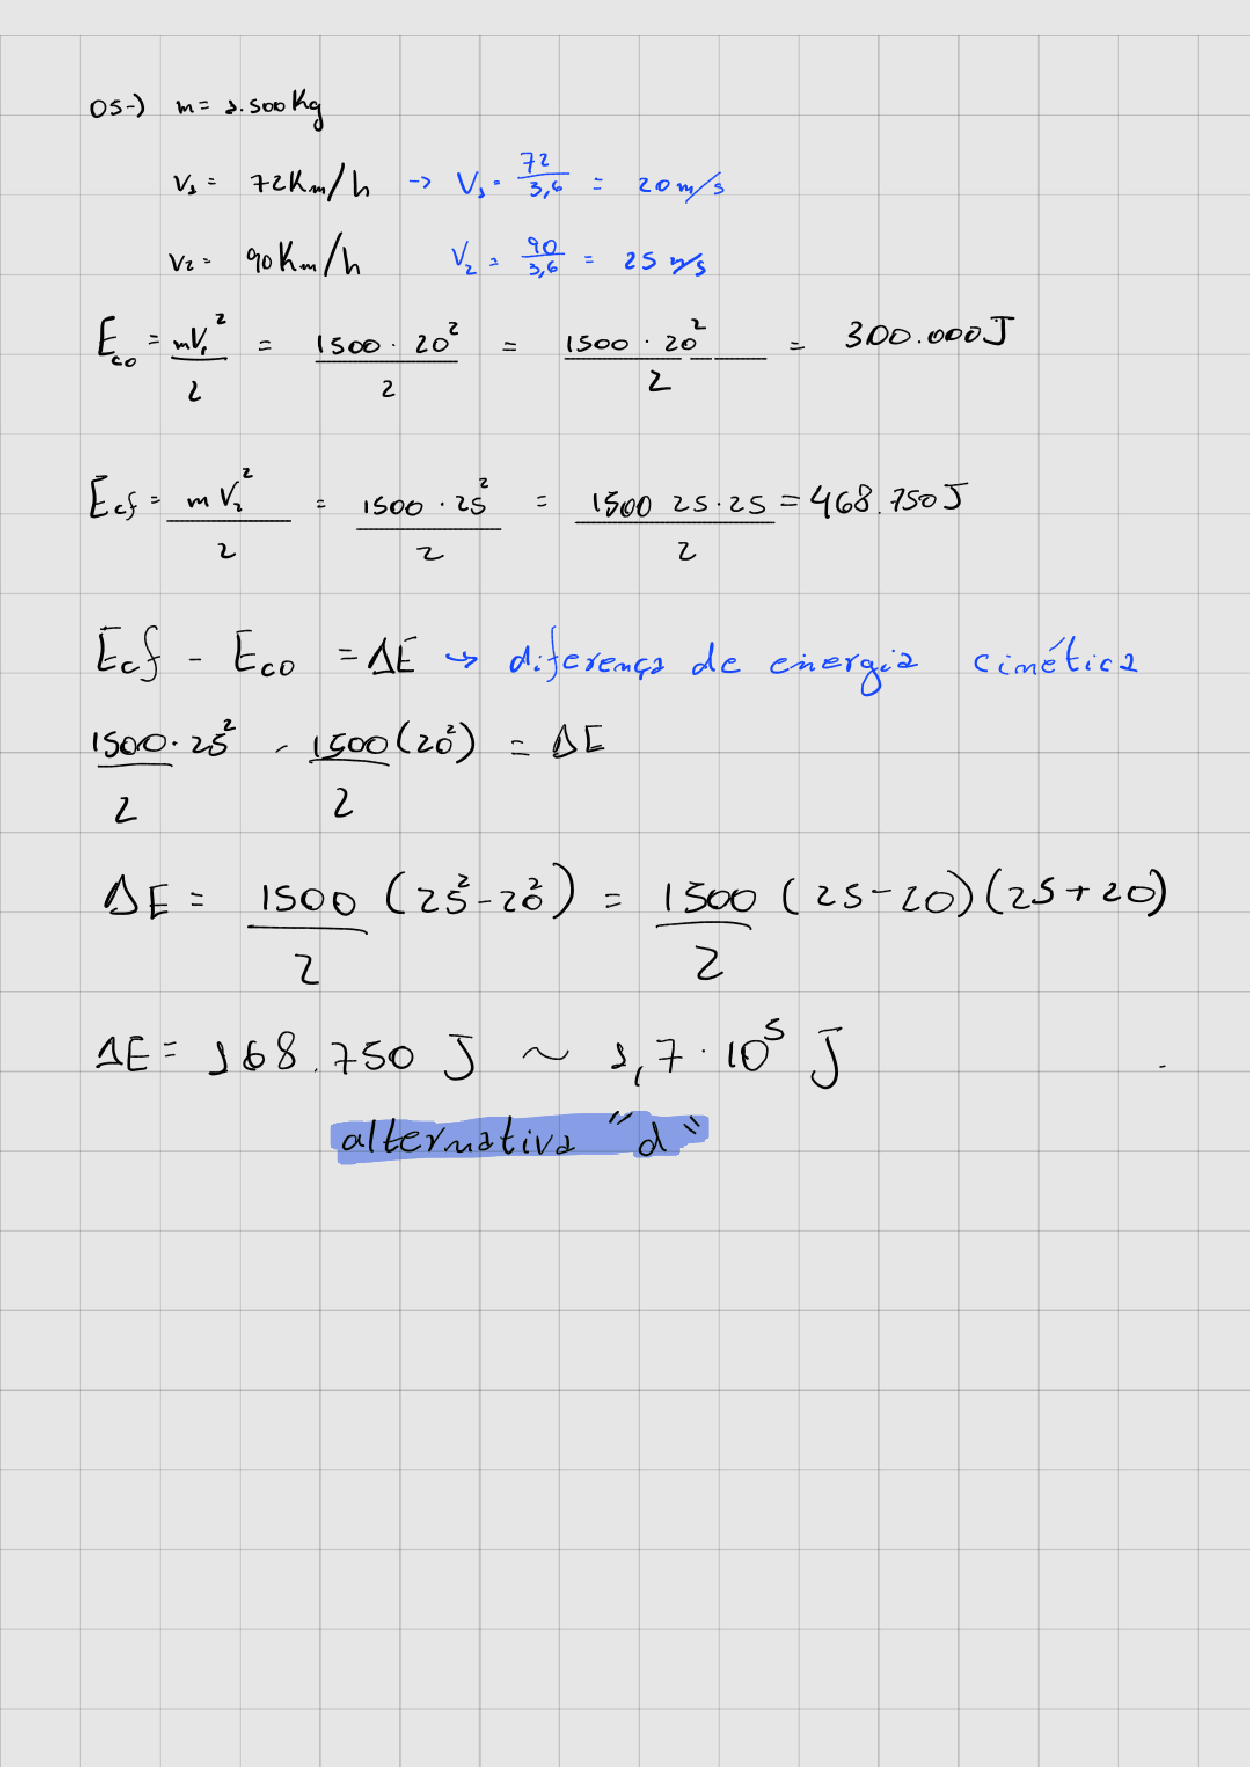
\includepdf[pages=1, scale=0.85, offset=0 -1.4cm,
%   pagecommand=\tituloanexo]{resolucoes_trabalho_energia.pdf}
%
% \includepdf[pages=2-, scale=0.95,
%   pagecommand={\thispagestyle{empty}}]{resolucoes_trabalho_energia.pdf}

\end{document}
